%% Dit is de domeinanalyse: Composite Objects %%
%% Freek 26 september: Een derde domeinanalyse zou kunnen gaan over hoe om te
%% gaan met Composite objects (bijv. hoe grafisch weer te geven, hoe op te
%% slaan in de data structuur)

\documentclass[a4paper,11pt,final]{article}

\usepackage[english]{babel}
\usepackage{graphicx}
\usepackage{hyperref}
\hypersetup{ colorlinks = true, citecolor = blue,linkcolor = blue }
\usepackage[a4paper]{geometry}
\usepackage{titlesec}% added to change section headers, see newcommand definition.


\bibliographystyle{alpha}

		

\begin{document}
\selectlanguage{english}
\begin{titlepage}
	\vspace*{\fill}
	\begin{center}
		\textsc{\large VT - XMD integration}\\[0.5cm]
		\textsc{Stefan Versluys}\\ \textsc{\scriptsize 19/02/2015}\\[2.0cm]
	\end{center}
	\vspace*{\fill}
\end{titlepage}


\tableofcontents

\newpage

\section{VT - XMD}
\paragraph{}
This paper concerns about the way verification tools (VT) can be integrated
into or interact with the Xmas Model Designer (XMD). There are several
options but not clear which is the best, because of conflicts in their
requirements \& specifications, additional risks, increase of complexity
and fade of basic rules concerning separation. 


\paragraph{VT requirements \& specification which affect integration decision:}
\begin{itemize}
\item The VT’s are written in pure c++ because they can run on platforms without any specific software tools.
\item VT’s their mayor key is performance.
\item The VT parser can handle a flat json structured file.
\item The VT parser cannot handle composites.
\item The VT parser feeds the VT model and has no GUI properties.
\item The VT’s can be started and get their input via the command prompt. (standalone)
\item The VT’s can be started and get their input via the designer tool.
\item The VT’s structure is complex because its focus is performance and not maintainability.
\item The VT’s give feedback via the standard output
\end{itemize}

\paragraph{XMD requirements \& specification which affect integration decision:}
\begin{itemize}
\item XMD is written in qml/c++ with Qt classes which gains development speed, fancy GUI, easy scripting.
\item XMD must handle composites.
\item XMD its major key is maintainability
\item Composites can be inside other composites and implies a hierarchical structure
\item XMD needs a hierarchical json parser
\item XMD needs GUI specific component properties like x,y,orientation
\item XMD doesn’t need VT specific component model data structures.
\item XMD must be pure GUI and doesn’t need to know about complex VT structures
\item Ideally VT integration in XMD must be purely interaction,  as if they are one thing for the XMD user but technically totally separated.
\item XMD must show the VT’s feedback in the console (normal text message)
\item XMD can show the VT’s result in the model (structured text message)
\end{itemize}

\paragraph{Team:}
\begin{itemize}
\item VT’s are out of scope.
\item Modifying VT’s parser and the structure to pass additional data is a risk:
	\begin{itemize}
	\item planning : complexity gains time?
	\item focus is XMD : loss of VT requirements/correctness?
	\item Because of OU changes, Bernard cannot be part of the team as developper.
	\item XMD interaction is done through the whole structure and makes VT and XMD very dependent from each other.
	\item Because of this dependence a change at the VT side can harm XMD and vice versa and breaks the maintainability rule.
		The same holds if changing XMD 
	\end{itemize}
\item	Using the VT parser and underlaying data structure extends the complexity into XMD which conflicts with its maintainability requirement.
\item Bernard: use only one data model, easier to maintain.
\item Bernard: VT has a parser you can use it.
\item Freeks concern of diving too deep into the VT’s because of too many risks and out of our scope. (see email)
\end{itemize}

\section{Options}
\paragraph{}

\paragraph{VT pure c++ parser only:}
\begin{itemize}
\item + only one file type for XMD and VT
\item +/- one parser and model : not an advantage see remarks (*)
\item - flattening must be done at VT side in pure c++
\item - XMD depends on the VT parser and complex VT structure for mapping.
\item - increased exposure to change issues between VT and XMD.
\item - VT structure mixed with GUI parameters (x,y,orientation,scale,..)
\item - VT parser and structure modification = risk + out of scope
\item - current fjson files not compatible anymore = loss of test references
\item - composites need to be handled/flattened in VT parser
\item - handling composite file locations, XMD vs. VT standalone on a pure platform
\item - id references of components or ports can become inconsistent.
\end{itemize}

(*)The advantage of having a parser already is not an issue because in
javascript a parser is one line of code.
The disadvantage of having to modify two parsers /models isn’t an issue
because in javascript, modifying is just adding a key/value and simple mapping.
If VT and XMD are independent, a modification of the XMD parser doesn’t lead to
a VT parser modification if it’s just about a GUI parameter, flattening can skip these.

\paragraph{XMD Javascript parser + VT dependent:}
\begin{itemize}
\item + XMD can have its own json structure with GUI specific parameters
\item + flattening can be done outside VT, no need to use pure c++
\item + fjson stays compatible
\item + no need to modify VT to handle composites (parsing+flattening)
\item + composite handling not necessary in VT for this project.
\item - two file types , one hierarchical json and one fjson. Same as the current WickedXmas.
\item - mapping for flattening is still done via VT parser/data, meaning complex VT data structures into flattener.
\item - a designer must hand over flat files to a verifier using VT as stand alone. 
\end{itemize}

\paragraph{XMD Javascript parser + VT independent:}
\begin{itemize}
\item same advantages as previous
\item + flattening done totally independant in e.g. Javascript , no need to know VT data structures.  No mapping
\item + XMD and VT are completly independent, only the fjson structure is common.
\item +/- flat structure in XMD must match VT flat structure , but in javascript
	very small modification. Much easier than adopt mapping to complex datastructures.
\item + flattening in the design tool can be used to see if there are no cycles before these are send to de VT’s
\item + very low risk, only the fjson structure must match
\item + no need of complex mapping code in designer, pure compact, robust and easy javascript
\item - two file types xmd + fjson
\item - XMD needs and SaveAs or export function to fjson , so VT’s can run models as standalone
\end{itemize}


\begin{figure}[here]
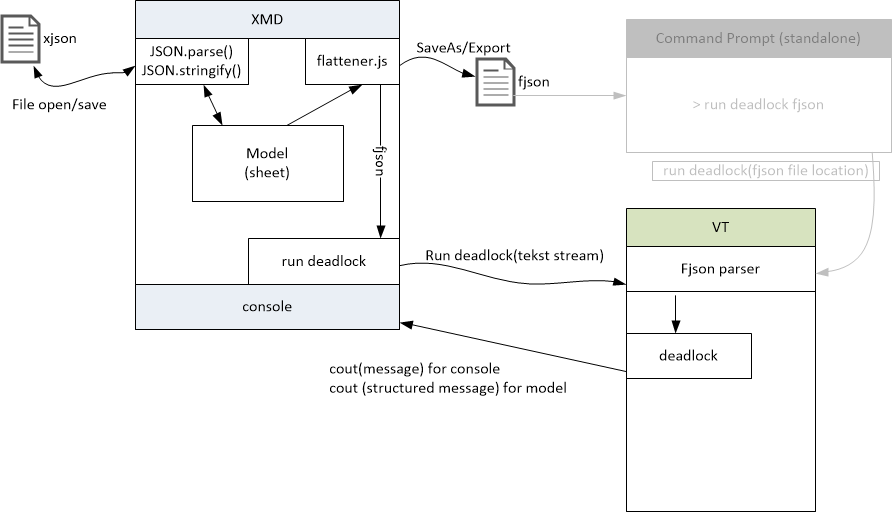
\includegraphics[width=1.0\textwidth]{xmd2vt}
\caption{vt to xmd interaction}
\label{fig:xmd2vt}
\end{figure}
Figure~\ref{fig:xmd2vt} is a setup where VT and XMD are totally independent
but can interact with each other as if they are one thing. By this XMD can keep
its maintainability and apart from minor changes VT stays untouched.
Teh fjson structure is the only key they have in common.



\end{document}